\documentclass[a4paper,11pt]{article}

% packages and settings [[[

% input	[[[
\usepackage[utf8]{inputenc}
\usepackage{ngerman}
% ]]]
% math/symbols [[[

\usepackage{latexsym}
\usepackage{amsfonts}	
\usepackage{amsmath}
\usepackage{amssymb}

% \usepackage{wasysym}	\Smile
% ]]]
% tables/graphics/algorithms/listings [[[

\usepackage{booktabs}
\usepackage{multirow}
\usepackage{graphicx}
\usepackage{listings}
\usepackage{algorithmic}
\usepackage[boxed]{algorithm}
\usepackage{subfigure}
\usepackage[margin=10pt,font=small,labelfont=bf]{caption}		
	% \caption zb. in \figure wird \small

% settings for listing environment
\lstset{language=C++,
		basicstyle=\small,
		frame=single,
        breaklines=true,
        breakatwhitespace=true,
		numbers=left,
		numberstyle=\tiny,
		xleftmargin=5mm,
		tabsize=4
}

% nicer comment formatting in algorithmic env.
\renewcommand{\algorithmiccomment}[1]{\hspace{\stretch{1}}// #1$\quad$}
\floatname{algorithm}{Algorithmus}

% drawin trees
% \usepackage{pstricks,pst-node,pst-tree}

% ]]]
% paragraph formatting [[[
% \usepackage{a4wide}

\usepackage{parskip}
\parindent0pt
\setlength{\parskip}{1ex plus 0.5ex minus 0.2 ex}

% ]]]

% ]]]
% my commands [[[

% my math commands [[[

\newcommand{\R}{\mathbb{R}}
\newcommand{\N}{\mathbb{N}}
\newcommand{\mts}{\;|\;}
\newcommand{\eqs}{\;=\;}
\newcommand{\D}{\mathrm{d}}
\newcommand{\Z}{\mathbb{Z}}
\renewcommand{\P}{\mathbb{P}}
\newcommand{\area}{\mathrm{area}}
\newcommand{\matrixtwo}[2]{\left(\begin{array}{cc}#1\\#2\end{array}\right)}
\newcommand{\matrixthree}[3]{\left(\begin{array}{ccc}#1\\#2\\#3\end{array}\right)}
\newcommand{\matrixfour}[4]{\left(\begin{array}{cccc}#1\\#2\\#3\\#4\end{array}\right)}
\newcommand{\vect}[3]{\left(\begin{array}{c}#1\\#2\\#3\end{array}\right)}
\newcommand{\vectfour}[4]{\left(\begin{array}{c}#1\\#2\\#3\\#4\end{array}\right)}
\newcommand{\norm}{\mathrm{norm}}
\newcommand{\scalPr}[2]{\left\langle #1|#2 \right\rangle}

% ]]]
% definitions [[[

\newcounter{currdefinition}
\newcommand{\defnr}[1]{\arabic{#1}}
\newcommand{\defref}[1]{Definition \defnr{#1}}
\newcommand{\definition}[2]
	{	\addtocounter{currdefinition}{1}%
		\newcounter{#1}%
		\setcounter{#1}{\thecurrdefinition}%
		\label{#1}%
		\paragraph{\textbf{Definition \thecurrdefinition:}}\ \\#2}

% ]]]
% misc commands [[[

\newcommand{\ra}{$\rightarrow\ $}
\newcommand{\wichtig}[1]{\framebox{\begin{minipage}[h]{\textwidth}#1\end{minipage}} }
\newcommand{\nachvollz}[1]{\paragraph{\textbf{Nachvollziehen:}}\ \\#1}
\newcommand{\tableitemization}{\hspace{10pt}$\bullet$&}
\newcommand{\HELP}[1]{\ \\\ \\\Huge Hilfe! \normalsize\\$\rightarrow$\ #1\ \\\ \\}

\newcommand{\inlinecode}[1]{{\tt #1}}
\newcommand{\inlineshell}[1]{{\tt #1}}

% ]]]
% levels [[[

\newcommand{\levelA}[1]{\section{#1}}
\newcommand{\levelB}[1]{\subsection{#1}}
\newcommand{\levelC}[1]{\subsubsection{#1}}
\newcommand{\levelD}[1]{\paragraph{#1:}\ \\}
\newcommand{\levelDn}[1]{\paragraph{#1:}}    % level D ohne "\ \\" --> bei paragraph oder itemization direkt danach sonst zu großer zwischenraum
\newcommand{\levelE}[1]{\paragraph{#1:}\ \\}
\newcommand{\levelEn}[1]{\paragraph{#1:}}    % level D ohne "\ \\" --> bei paragraph oder itemization direkt danach sonst zu großer zwischenraum

% ]]]

% ]]]

\usepackage{url}
\usepackage{a4wide}

\title{Messungen}
\author{Kai}
\date{\today}

% \setlength{\unitlength}{1mm}

\begin{document}

\maketitle\thispagestyle{empty}
% \tableofcontents
Bestimmte Messungen sind im Git eingecheckt. Hier soll stehen was sie tun und wie das Ergebnis aussieht.

\section{Einfache BBVHs und SBVHs \hfill 2012-07-04}

Alle Messungen auf Istar\marginpar{Istar}.

\newcommand\Cis{\texttt{Cis}\ }
\newcommand\Dis{\texttt{Dis}\ }
\newcommand\cis{\texttt{cis}\ }
\newcommand\dis{\texttt{dis}\ }
\newcommand\newword[1]{\marginpar{#1}}
\newcommand\frage{\marginpar{\tt \Large ?}}
\newcommand\todo{\marginpar{\tt \Large Todo!}}
\newcommand\file[1]{{\tt #1}}

\newword\dis
\Dis ist die naivste Traversionmethode: 
	Wird ein Knoten getroffen werden die Kinder (immer das linke zuerst) ohne nähere Betrachtung auf den Stack gelegt.
\newword\cis
\Cis ist die Traversion bei der anstatt die Box des eigentlichen Knotens die beiden Boxen der Kinder geschnitten werden. 
	Es werden nur Kindknoten auf den Stack gelegt, die auch tatsächlich getroffen wurden, und wenn beide Kinder
	getroffen werden, wird das am weitesten entfernte zuerst auf den Stack gelegt.

Offensichtlich ist die Performance von \dis abbhängig von der Richtung aus der auf die Szene geschaut wird.
Im besten Fall wird immer genau der Knoten zuerst auf den Stack gelegt, der dem Strahl am nähesten ist, 
	im schlechtesten Fall immer derjenige, der am weitesten weg ist (was Pruning) effizient verhindert.

Offene Frage: \frage wie sieht es aus, wenn nicht von außen auf die Szene geschaut wird, sondern von innen heraus, z.B. im Conf-Room eine
	sphärische Messung vom Mittelpunkt aus?
Könnte sein, dass der Performance-Vorteil beim Render aus der Best-Case Richtung dadurch verringert wird.

Die Messreihe umfasst 642 Bilder der Form:
\begin{center}

\includegraphics[width=\textwidth]{messreihe-bsp.png}
\end{center}

Das Skript zu den Messungen (sowie die Messergebnisse selbst) liegt unter \url{messungen/2012-07-04/}.

Gemessen wurden folgende Vergleiche:
\begin{itemize}
\item \file{dis-rel-to-cis}:
	Performance von \dis relativ zu \cis (also \cis/\dis), auf der guten Seite ist \dis $3.9$\% schneller, 
	insgesamt erreicht es aber nur $66.5$\% der Performance.
\item \file{sbvh-cis-rel-to-cis} und \file{sbvh-dis-rel-to-dis}:
	Es wird jeweils die generische Stackless-Bvh und die normale BBVH mit \cis bzw.\ \dis gemessen.
	Der Vergleich zeigt, dass die Struktur allein keinen Unterschied macht (was auch nicht überrascht).
\item \file{sbvh-po-rel-to-cis}:
	Der wirklich interessante Vergleich: die postorder Stackless-Bvh relattiv zu \cis.
	\begin{center}
	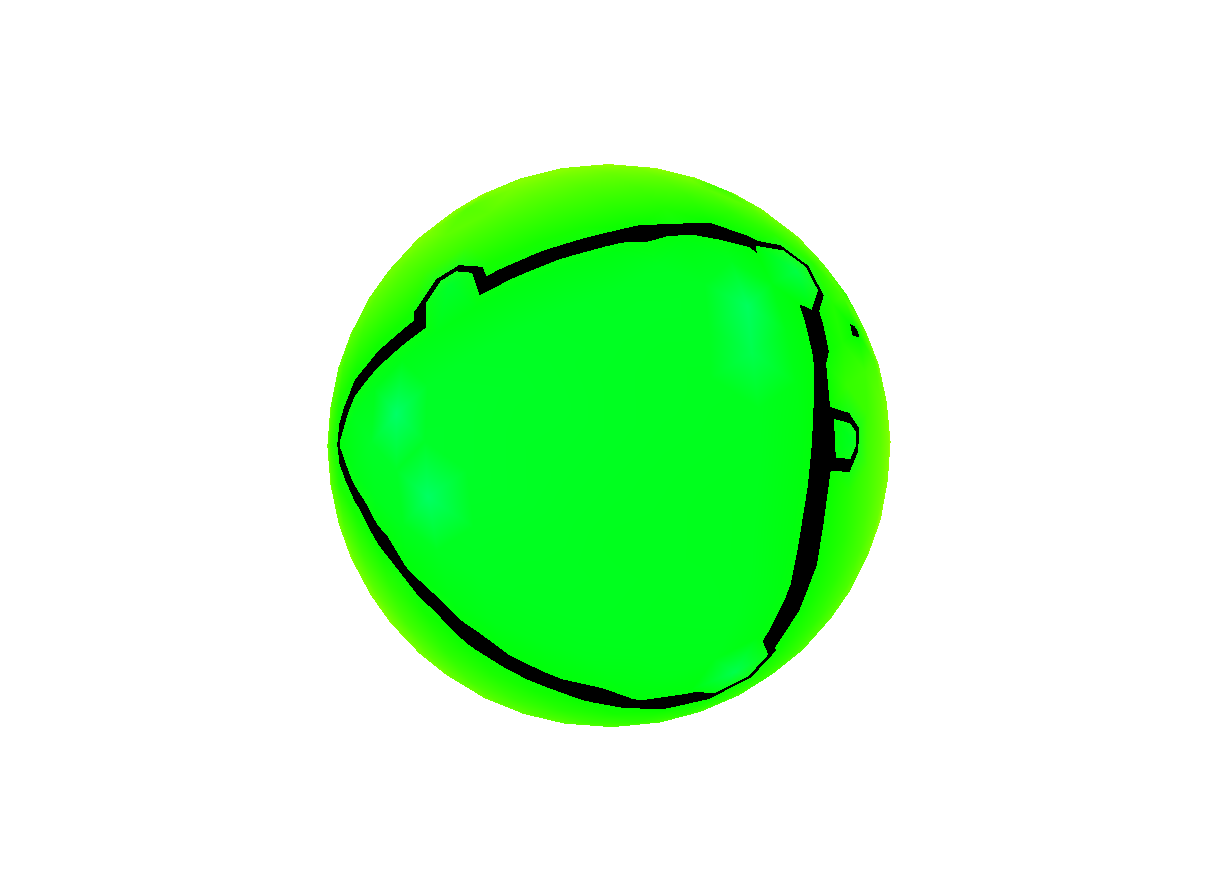
\includegraphics[width=.45\textwidth]{2012-07-04/sbvh-vs-bbvh-good.png}\hfill
	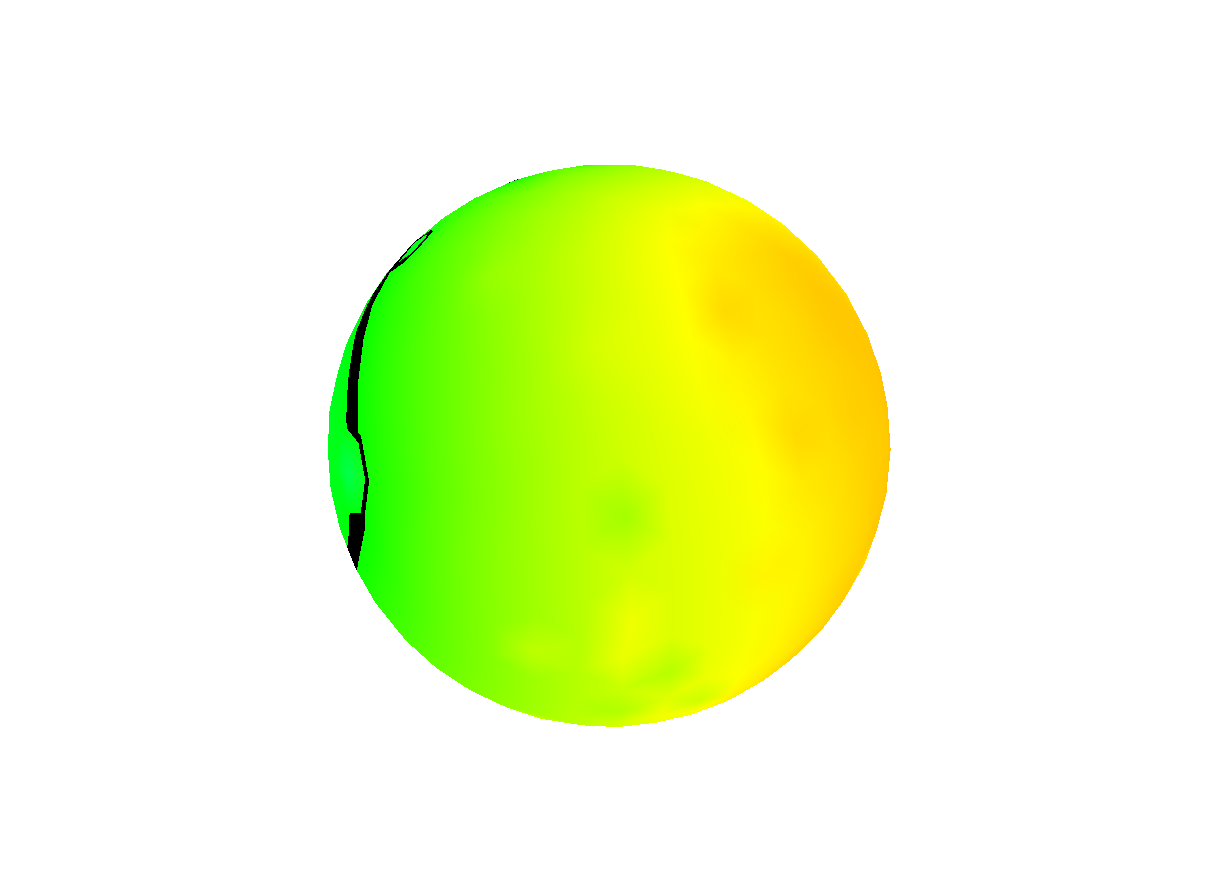
\includegraphics[width=.45\textwidth]{2012-07-04/sbvh-vs-bbvh-ramp.png}
	\end{center}
	Auf dem ersten Bild ist kaum ein Unterschied zu erkennen, der schwarze Rahmen markiert wo beide etwa gleich auf sind, im inneren Bereich ist die
	stackless Variante etwas schneller.
	Das zweite Bild zeigt, dass der Performance außerhalb der optimalen Richtung stark abfällt.
\item \file{sbvh-po-masked-good-part}, \file{bbvh-dis-masked-good-part} und \file{bbvh-cis-marked-same-part}:
	Hier wurde der ``gute'' Oktant extrahiert und die Performance für die drei Varianten verglichen.
	Wie oben erwähnt ist \dis in dem Bereich $3.9$\% schneller als \cis.
	Die stackless Variante kommt auf 6\%.

	Hier ein Beispiel für die maskierten Kugeln:
	\begin{center}
	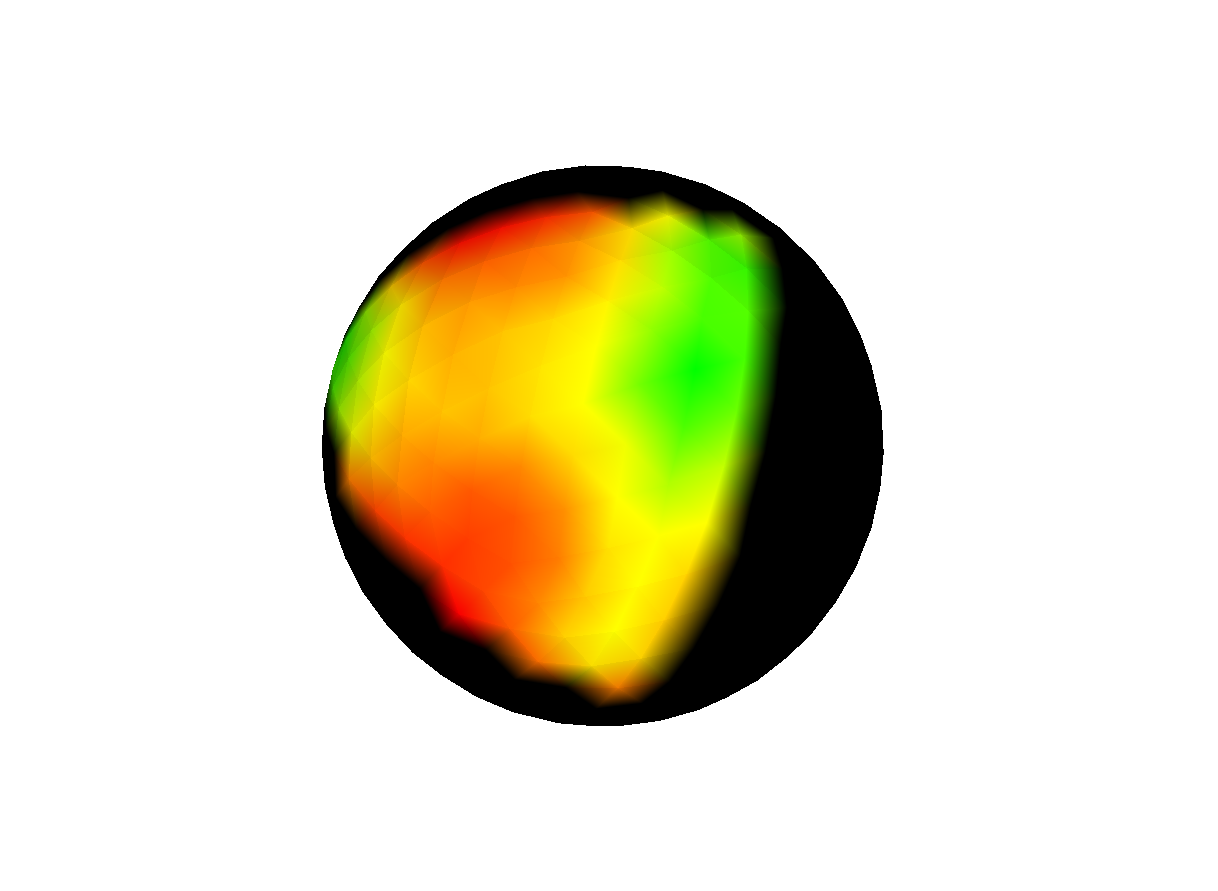
\includegraphics[width=.45\textwidth]{2012-07-04/masked-sphere.png}\hfill
	\end{center}

\end{itemize}

Bis auf die letzte Messung sind alle Messungen in dem beiden Shellskripten abgelegt.
Die letzte wurde wiefolgt durchgeführt:

{\small
\begin{verbatim}
$ sphs 2012-07-04--E--sbvh-po-sbvh.ply -m mask -O -1,-1,-1 -o sbvh-po-masked-good-part.ply
...
$ sphs 2012-07-04--A--bbvh-dis.ply -m mask -O -1,-1,-1 -o bbvh-dis-masked-good-part.ply
...
$ sphs 2012-07-04--B--bbvh-cis.ply -m mask -O -1,-1,-1 -o bbvh-cis-masked-same-part.ply
...
$ sphs bbvh-cis-masked-same-part.ply -m check
bbvh-cis-masked-same-part.ply: average of 2437.66 krps, [ 2090.49 : 2882.08 ]
$ sphs sbvh-po-masked-good-part.ply -m check
sbvh-po-masked-good-part.ply: average of 2299.54 krps, [ 2038.42 : 2725.35 ]
$ sphs bbvh-dis-masked-good-part.ply -m check
bbvh-dis-masked-good-part.ply: average of 2390.23 krps, [ 1944.38 : 2871.17 ]
\end{verbatim}}

\end{document}

% vim: set foldmethod=marker foldmarker=[[[,]]]: 


